\section{Numerical Results}
  \label{sec:twophoton_results}

  \subsection{Weak Beam Spectra}

    Before we investigate the effect of a strong field on the atomic medium, it
    is useful to look at the results of an applied field in the weak probe
    regime. As discussed in chapter \ref{chp:propagation}, in the weak field
    limit it is possible to derive analytic expressions for the spetral
    Lorentzian (or Voigt, when broadened)  lineshape corresponding to the
    imaginary part of the coherences and thus for the expected absorption
    profiles.

    The \textit{ElecSus} software package\cite{Zentile2015} calculates
    transmission and susceptibility spectra for weak probes in thermal alkali
    metal vapours, in excellent agreement with experimental
    data.\cite{Siddons2008,Weller2011} We use this tool as a reference with
    which to compare the results for our model at weak field, before we take our
    model beyond the constraints of the weak probe regime.

    \begin{figure}[]
    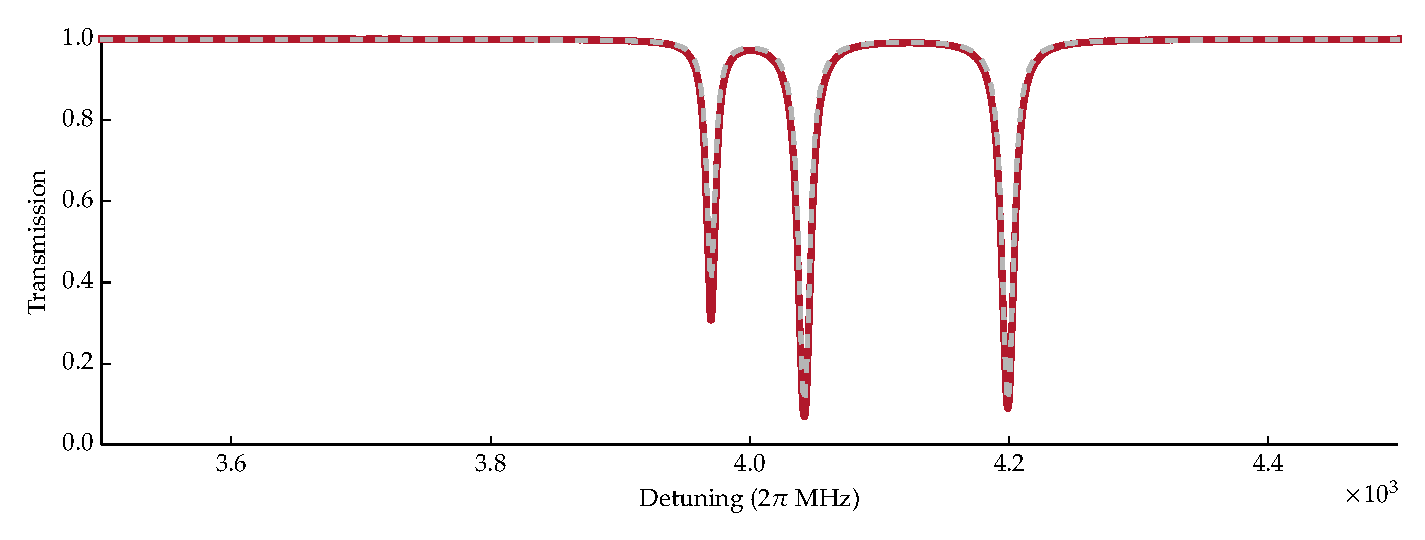
\includegraphics[width=\linewidth]
        {figs/05_twophoton/rb87_d2_hf_solve_scan_g2a_fig3.pdf}
    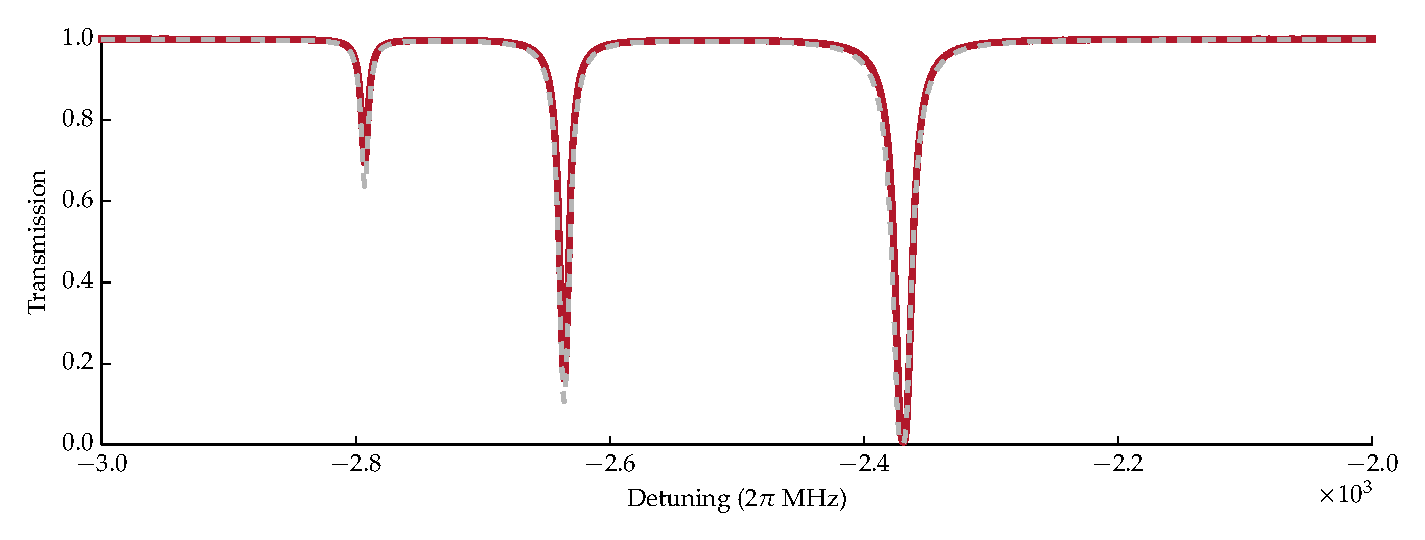
\includegraphics[width=\linewidth]
        {figs/05_twophoton/rb87_d2_hf_solve_scan_h1a_fig3.pdf}
    \caption{
    Simulated transmission (red) of a weak ($I~=~\unit[10^{-6}]{W~cm^{-2}}$)
    probe beam scanned across the  $F = 1 \rightarrow F$ \textsc{d2} lines in a
    \unit[1]{cm}long vapour cell of rubidium 87 is compared with the result of
    the ElecSus program (grey dashed). Doppler broadening is neglected and the
    number density $N = \unit[7.5\cdot10^{15}]{m^{-3}}$. The simulated transit
    time \unit[2]{$\mu$s}.
    }
    \label{fig:weak_d2} 
    \end{figure}

    In figure \ref{fig:weak_d2} we show the results of a simulated scan of a
    weak probe (with intensity $I = $\unit[$10^{-6}$]{W cm$^{-2}$}) with no
    Doppler broadening, corresponding to a temperature close to \unit[$0$]{K},
    but with a number density of $N = \unit[7.5\cdot10^{15}]{m^{-3}}$,
    corresponding via  vapour pressure equations\cite{Zentile2015} to a
    temperature $T = \unit[20]{\text{\textdegree C}}$. The removal of broadening
    is an artificial constraint intended to separate the Lorentzian lineshape of
    the coherence terms (and thus absorption profile) without needing to include
    the Gaussian convolution. The simulated length of the medium in this case is
    \unit[1]{cm}.

    The top subplot covers the transition from ground state hyperfine levels $F
    = 1$ to excited state hyperfine levels $F' = \{ 0, 1, 2 \}$ and the bottom
    subplot covers the transition from hyperfine levels $F = 2$ to excited state
    hyperfine levels $F' = \{ 1, 2, 3 \}$. We see good agreement between the
    optical Bloch model and the ElecSus result for the positions, widths and
    amplitudes of the absorption troughs.

    To obtain spectra for closed systems it is typical to compute the density
    matrix elements in the steady state, \ie by setting  $\partial \rho /
    \partial t = 0$ in the Lindblad master equation (\ref{eqn:lindblad}). This
    requires less computation than integrating the differential equations over
    time, but is not possible in this system because of hyperfine pumping. As $t
    \rightarrow \infty$, all of the population is pumped to the other ground
    state. Instead, we solve the master equation over a range of detunings up to
    an average transit time of atoms in the beam, in this case \unit[2]{$\mu$s},
    and take the resulting density matrix elements at this point in the time
    evolution.

    \begin{figure}[]
    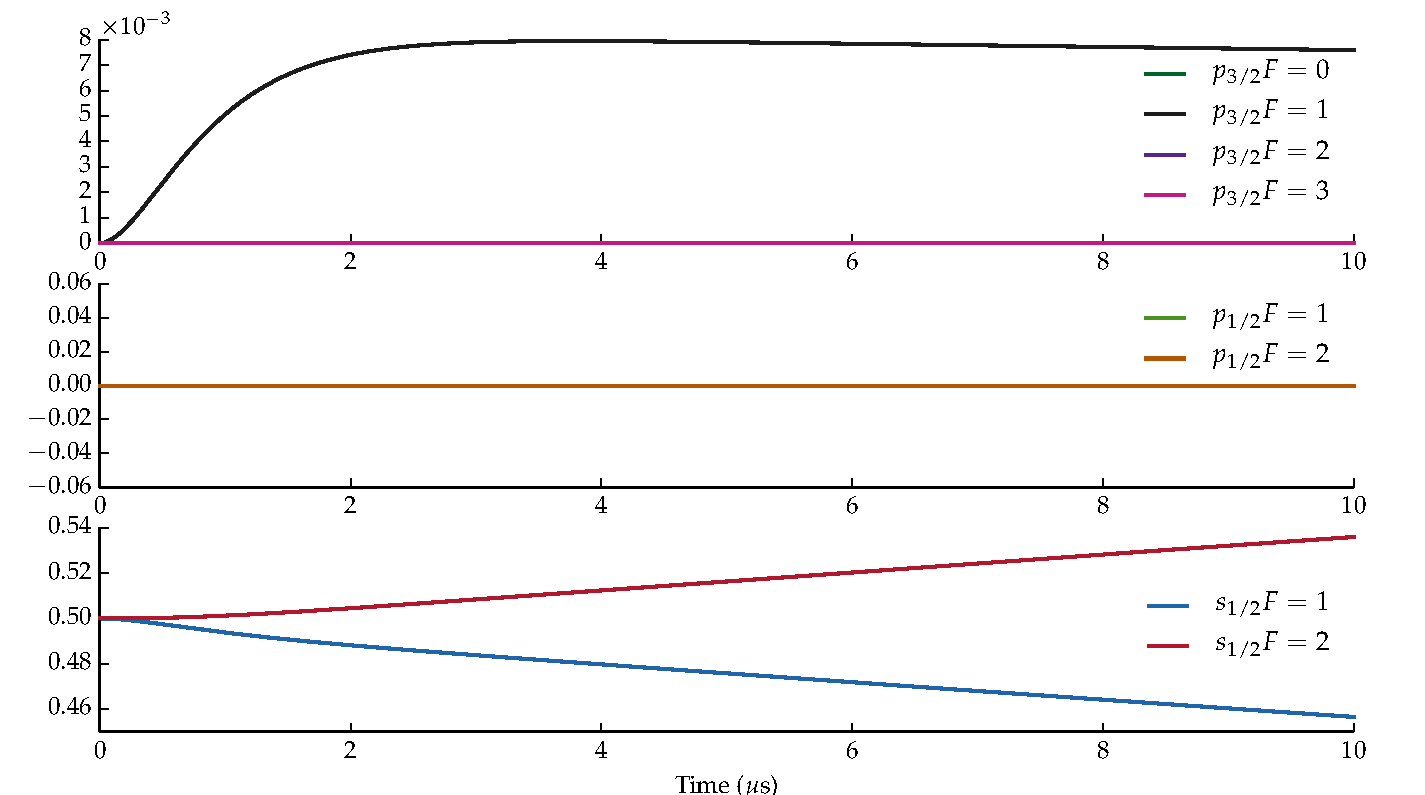
\includegraphics[width=\linewidth]
        {figs/05_twophoton/rb87_5spd_hf_solve_b0_fig1.pdf}
    \caption{
    Populations of the $^{87}$Rb $5\rm{P}_{\nicefrac{3}{2}}$ (top) and
    $5\rm{P}_{\nicefrac{1}{2}}$ (middle) excited states and
    $5\rm{S}_{\nicefrac{1}{2}}$ ground states (bottom)  after interaction with
    a weak ($I = $\unit[$10^{-6}$]{W cm$^{-2}$}) beam on resonance with the $F =
    1 \rightarrow F' = 1$ \textsc{d2} line over a period of \unit[10]{$\mu$s}.
    }
    \label{fig:weak_d2_f11} 
    \end{figure}

    Figure \ref{fig:weak_d2_f11} shows the populations of the hyperfine levels
    \begin{equation}
      \rho_{FF} = \sum_{m_F} \Tr \left[ \Ket{F m_F} \Bra{F m_F} \right].
    \end{equation}
    of the $5\rm{S}$ and $5\rm{P}$ states for one such detuning, on
    resonance with the $F = 1 \rightarrow F' = 1$ \textsc{d2} transition. As we
    would expect, we see that a small amount of population is driven from the $F
    = 1$ ground state to the $F' = 1$ excited state, reaching a peak at around
    \unit[3]{$\mu$s}. This excited population then begins to decrease over time
    as population is transferred from the $5\rm{S}_{\nicefrac{1}{2}} F = 1$
    ground state  to the $5\rm{S}_{\nicefrac{1}{2}} F = 2$ ground state by
    hyperfine pumping.

  \subsection{Strong Beam Spectra}

    Next we move beyond the weak-probe approximation to investigate the response
    of the atom is to a strong beam. Again we'll consider just the
    $5\rm{S}_{\nicefrac{1}{2}}$ ground state manifold and the
    $5\rm{P}_{\nicefrac{3}{2}}$ excited state manifold representing the
    \textsc{d2} transition.

    \begin{figure}%[]
    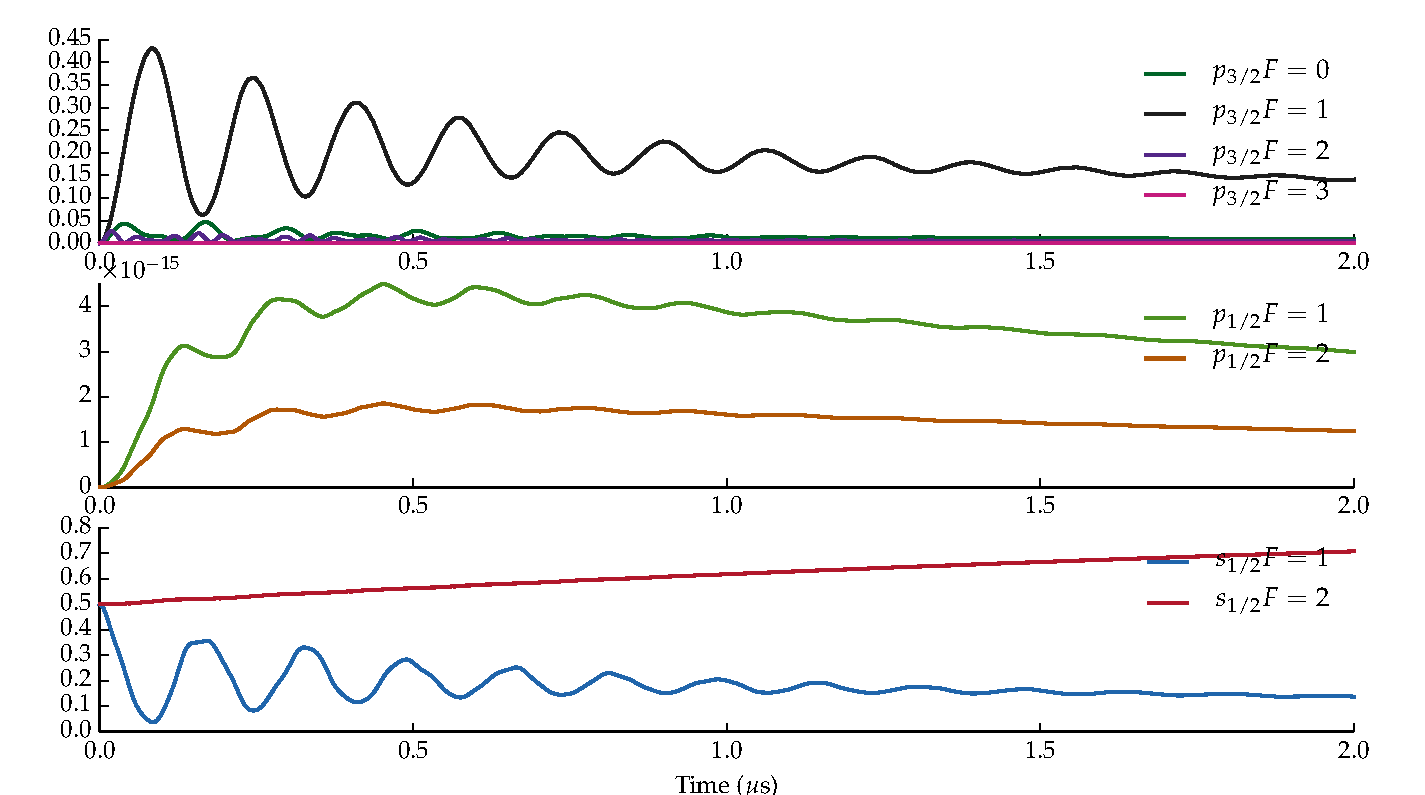
\includegraphics[width=\linewidth]
        {figs/05_twophoton/rb87_5spd_hf_solve_b3_fig1.pdf}
    \caption{
    Populations of the $^{87}$Rb $5\rm{P}_{\nicefrac{3}{2}}$ (top) and
    $5\rm{P}_{\nicefrac{1}{2}}$ (middle) excited states and
    $5\rm{S}_{\nicefrac{1}{2}}$ ground states (bottom)  after interaction with
    a strong ($I = $\unit[$1$]{W cm$^{-2}$}) beam scanned on resonance $F = 1
    \rightarrow F' = 1$ \textsc{d2} line over a period of \unit[2]{$\mu$s}.
    }
    \label{fig:strong_d2_f11} 
    \end{figure}

    \begin{figure}%[h]
    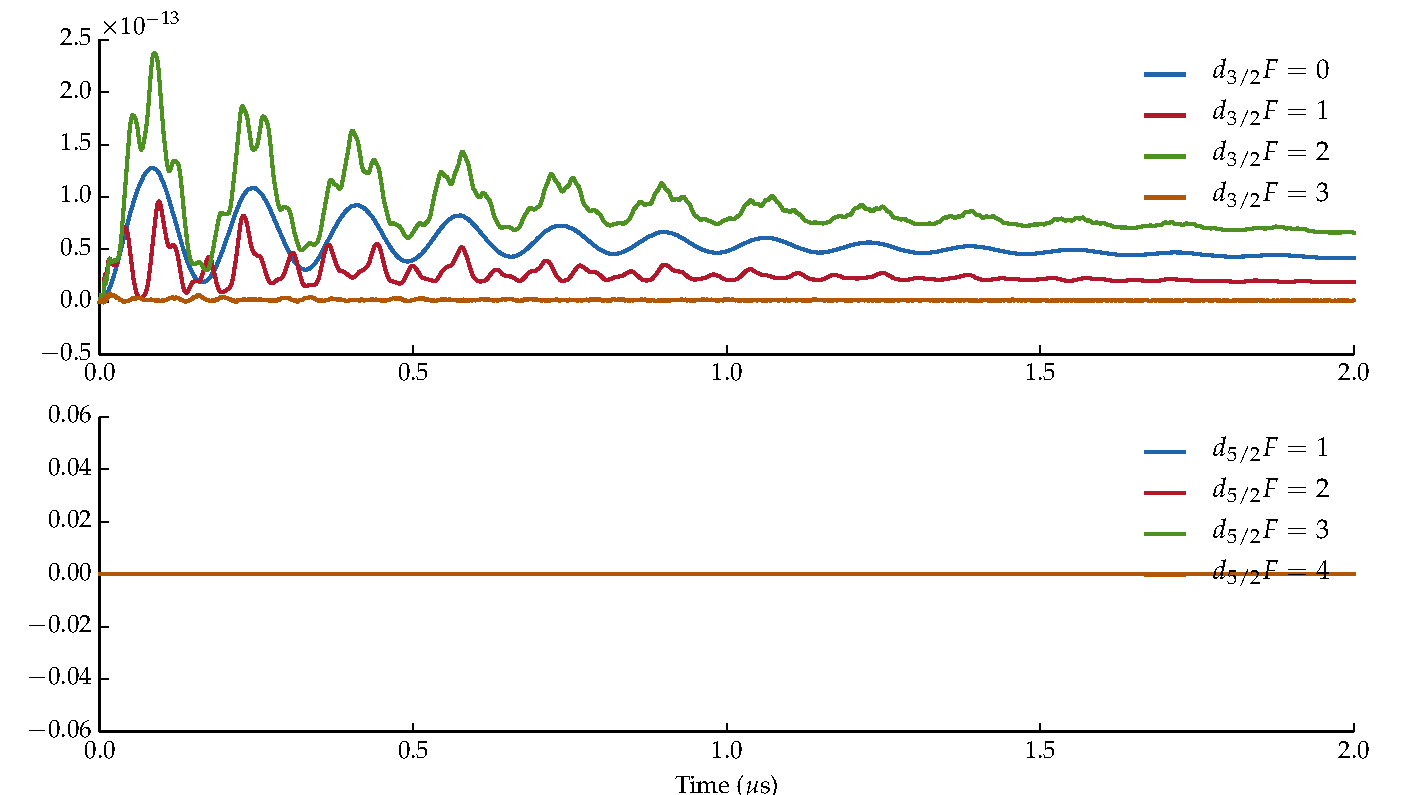
\includegraphics[width=\linewidth]
        {figs/05_twophoton/rb87_5spd_hf_solve_b3_fig2.pdf}
    \caption{
    Populations of the $^{87}$Rb $5\rm{D}_{\nicefrac{3}{2}}$ (top) and
    $5\rm{D}_{\nicefrac{5}{2}}$ (bottom) excited states for the same systems as
    figure \ref{fig:strong_d2_f11}.
    }
    \label{fig:strong_d2_f11_D} 
    \end{figure}

    Figures \ref{fig:strong_d2_f11} and \ref{fig:strong_d2_f11_D} show the
    system populations for a beam resonant with the same $F = 1 \rightarrow F' =
    1$ \textsc{d2} transition as figure \ref{fig:weak_d2_f11}, but at a stronger
    intensity of $I = $ \unit[$1$]{W cm$^{-2}$}. The population excited to the
    $5\rm{P}_{\nicefrac{3}{2}} F' = 1$ state is much higher, and now we see Rabi
    oscillations in the populations. Here we see two-photon excitation to the
    $5\rm{D}_{\nicefrac{3}{2}}$ state for the first time, albeit on the order of
    $10^{-13}$. Decay from the now populated $5\rm{D}_{\nicefrac{3}{2}}$ states
    to $5\rm{P}_{\nicefrac{1}{2}}$ means we also see population in the latter,
    which was not observed in the weak field solution shown in figure
    \ref{fig:weak_d2_f11}.

    \begin{figure}%[h]
    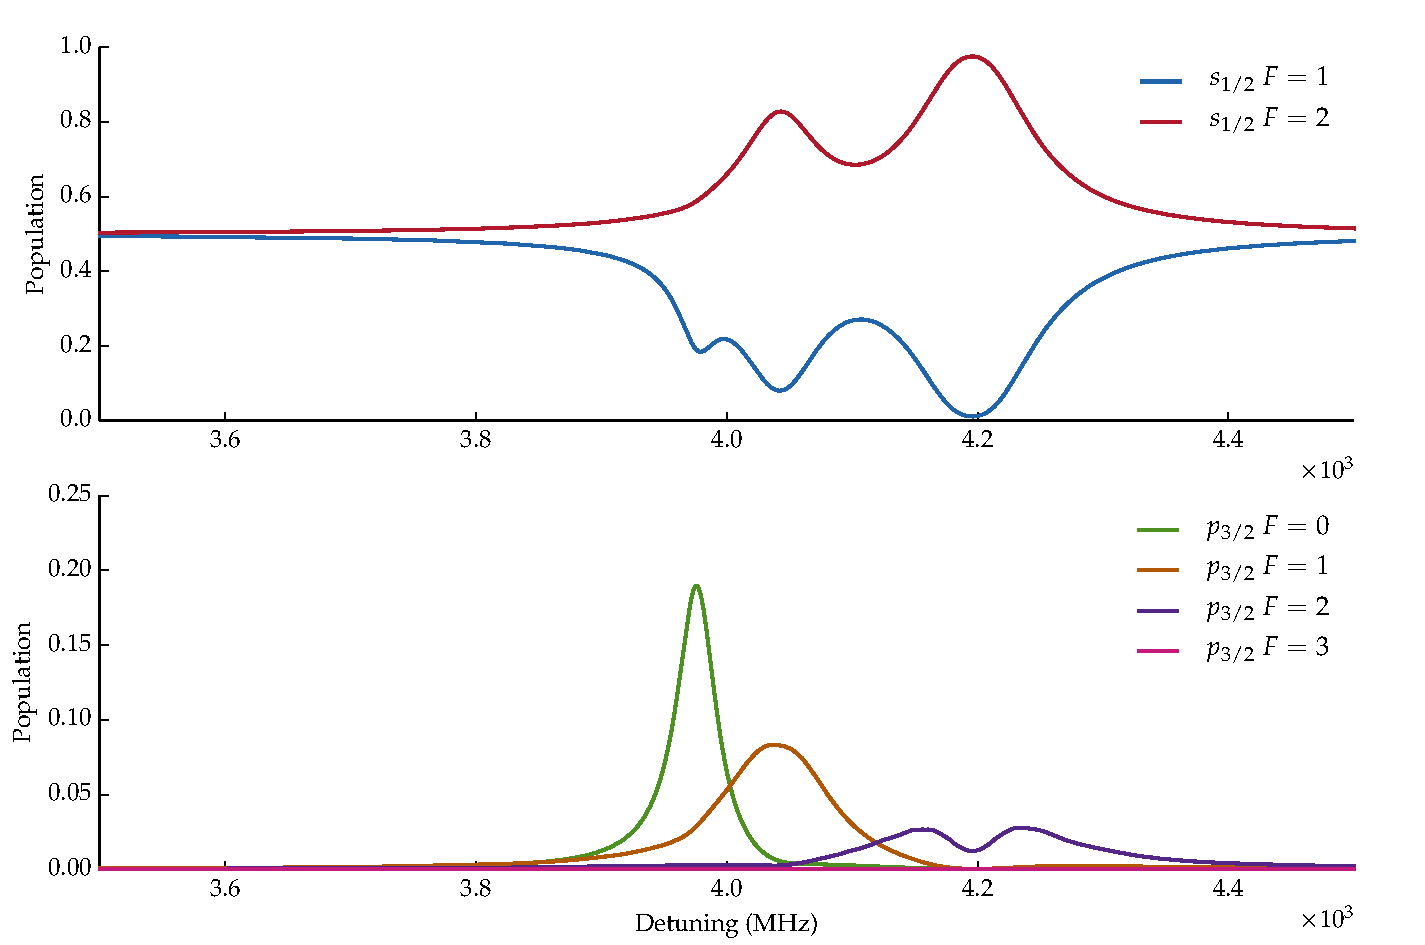
\includegraphics[width=\linewidth]{figs/05_twophoton/rb87_d2_hf_solve_scan_g3a_fig1.pdf}
    \caption{
    Populations of the $^{87}$Rb $5\rm{S}_{\nicefrac{1}{2}}$ ground states
    (top) and $5\rm{P}_{\nicefrac{3}{2}}$ excited states (bottom) after
    interaction with a strong ($I = $ \unit[$1$]{W cm$^{-2}$}) beam scanned
    across the $F = 1 \rightarrow F'$ \textsc{d2} lines with a transit time of
    \unit[2]{$\mu$s}.
    }
    \label{fig:strong_d2_f1} 
    \end{figure}

    \begin{figure}%[h]
    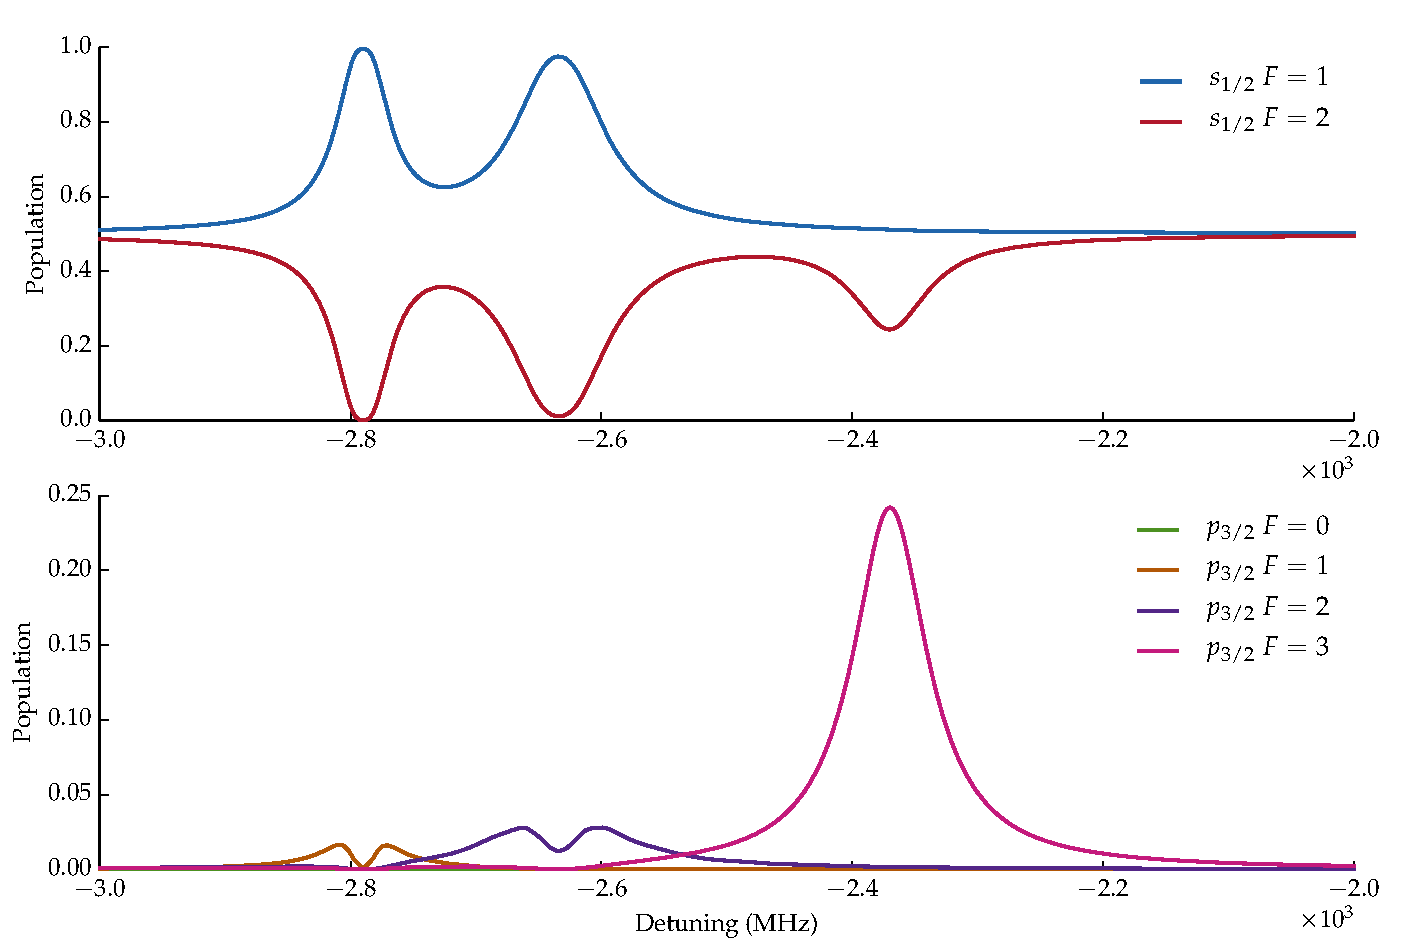
\includegraphics[width=\linewidth]{figs/05_twophoton/rb87_d2_hf_solve_scan_h2a_fig1.pdf}
    \caption{
    Populations of the $^{87}$Rb $5\rm{S}_{\nicefrac{1}{2}}$ ground states
    (top) and $5\rm{P}_{\nicefrac{3}{2}}$ excited states (bottom) after
    interaction with a strong ($I = $ \unit[$1$]{W cm$^{-2}$}) beam scanned
    across the $F = 2 \rightarrow F'$ \textsc{d2} lines with a transit time of
    \unit[2]{$\mu$s}.
    }
    \label{fig:strong_d2_f2} 
    \end{figure}

    In figures \ref{fig:strong_d2_f1} and \ref{fig:strong_d2_f2} we show the
    results of simulated scan, again over the \textsc{d2} lines of rubidium 87,
    but this time with a strong beam of intensity $I = $ \unit[$1$]{W
    cm$^{-2}$}. This is beyond the saturation intensity and in the regime where
    power broadening has a significant effect on the transmission profile. The
    transit time is again \unit[2]{$\mu$s}.

    In figure \ref{fig:strong_d2_f1} we show the populations of the hyperfine
    $5\rm{S}_{\nicefrac{1}{2}}$ ground states and
    $5\rm{P}_{\nicefrac{3}{2}}$ excited states as the probe is scanned across
    the $F = 1$ to $F' = \{ 0, 1, 2 \}$ transitions. We see that when we are far
    off-resonance the population remains in the initial state, evenly divided
    between the two ground state hyperfine levels. As the scan crosses the
    resonance lines we see population is removed from the $F = 1$ state and
    populates the excited hyperfine states according to that transition's
    relative transition strength. The lineshapes are now much broader than the
    natural linewidth due to power broadening\cite{loudon2000quantum}. The $F' =
    2$ population has a double- peaked lineshape. This is due to hyperfine
    pumping saturating this transition at this probe strength, \ie on resonance
    from $F = 1 \rightarrow F' = 2$ all of the population decays to the $F = 2$
    state within \unit[2]{$\mu$s} at this intensity such that the population in
    the $F' = 2$ state is limited.

    In figure \ref{fig:strong_d2_f2} we show the same populations as in figure
    \ref{fig:strong_d2_f1}, but for the probe scanned across the $F = 2$ to $F'
    = \{ 1, 2, 3 \}$ transitions. We again see that far off-resonance the
    populations remain in their initial condition state, evenly split between
    the two ground state hyperfine levels. As the scan crosses the resonance
    lines, this time we see conversely that the population is removed from the
    $F = 2$ state to populate the excited hyperfine states according to the
    transition strengths. This time it is the $F' = 1$ and $F' = 2$ transitions
    that are saturated by the hyperfine pumping such that the initial state
    population is limited on resonance after \unit[2]{$\mu$s} at this intensity.

  \subsection{Fluorescence with High-Intensity Beam}

    Now that we have investigated population of the
    $5\rm{S}_{\nicefrac{1}{2}}$ hyperfine ground states as the probe is
    scanned across the \textsc{d2} lines, both for a weak probe and a strong
    probe, we will move onto adding in the two-photon excited states ---
    firstly, the $5\rm{D}_{\nicefrac{3}{2}}$ and $5\rm{D}_{\nicefrac{5}{2}}$
    states coupled near resonance, and the $6\rm{P}_{\nicefrac{1}{2}}$ and
    $6\rm{P}_{\nicefrac{3}{2}}$ decay channels. Decay from the
    $6\rm{P}_{\nicefrac{1}{2}}$ state is the source of optical fluorescence at
    \unit[422]{nm}. We wish to observe if there is \textit{enough} population in
    these exited states through single-atom processes to account for the
    fluorescence shown in figure \ref{fig:blue_flourescence}.

    \begin{figure}%[h]
    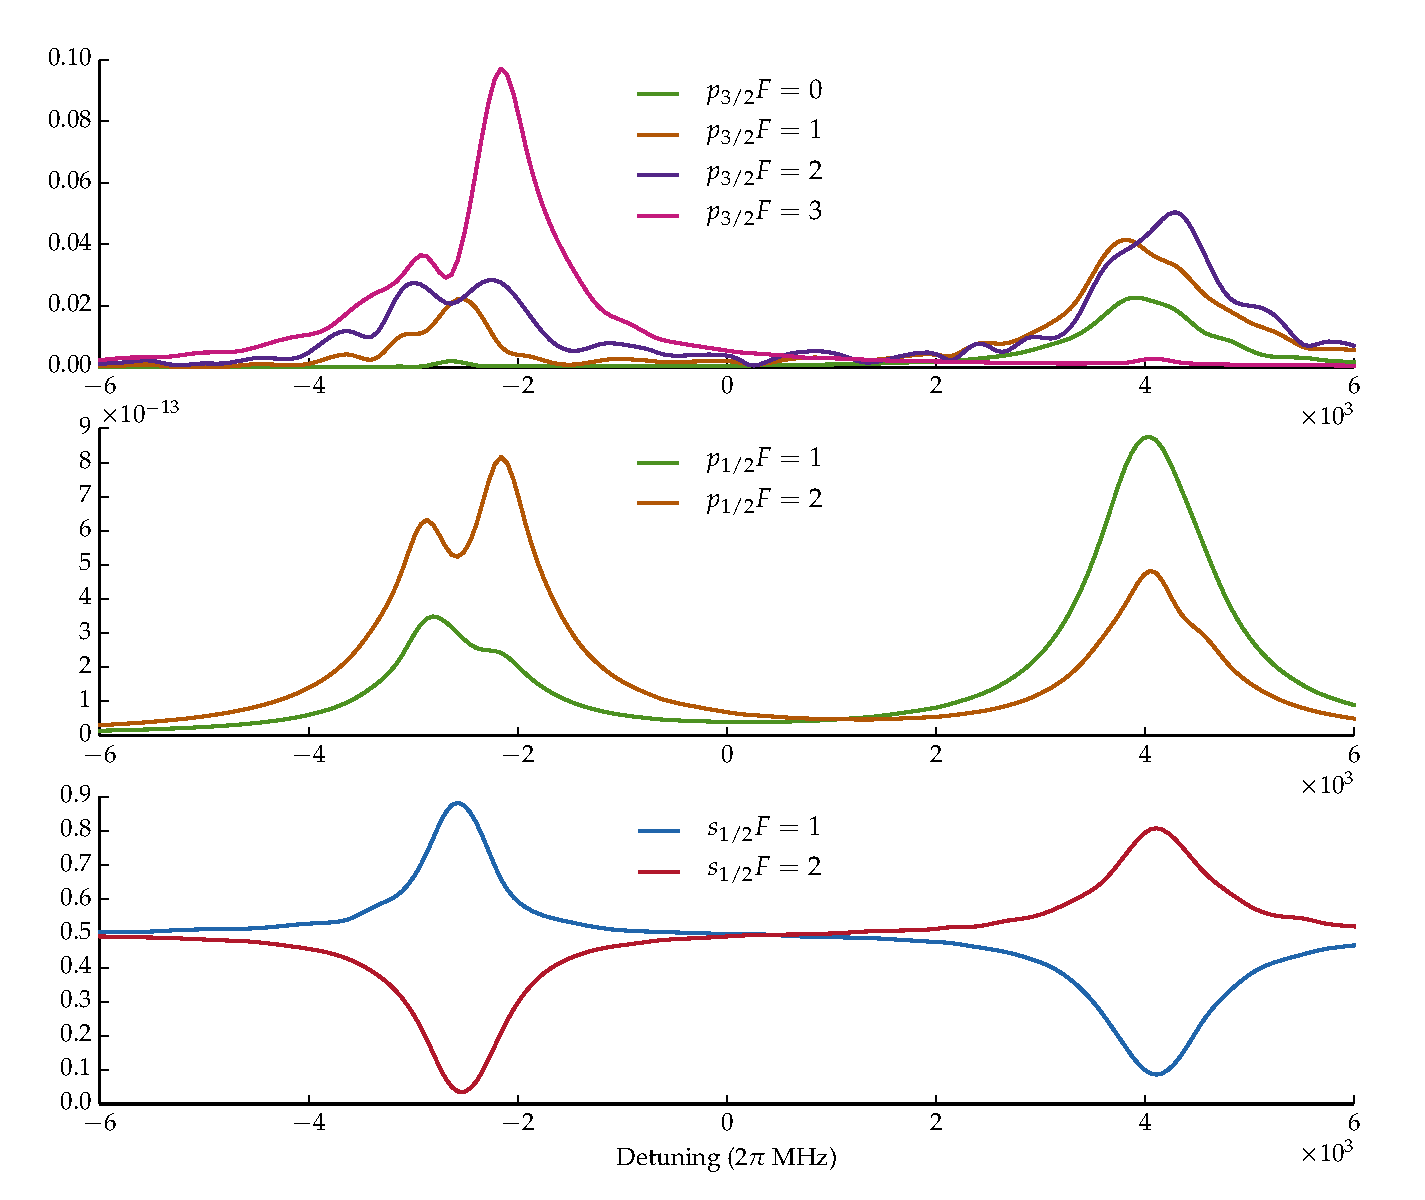
\includegraphics[width=\linewidth]{figs/05_twophoton/rb87_5spd6p_hf_2_solve_scan_e02_FIXED_1e2W_fig1.pdf}
    \caption{
    Populations of the $^{87}$Rb $5\rm{S}_{\nicefrac{1}{2}}$ ground states
    (bottom), $5\rm{P}_{\nicefrac{3}{2}}$ (middle) and
    $5\rm{P}_{\nicefrac{1}{2}}$  (bottom) excited states after interaction
    with a strong ($I = $ \unit[$10^2$]{W cm$^{-2}$}) beam scanned across the $F
    = 2 \rightarrow F'$ \textsc{d2} lines with a transit time of
    \unit[2]{$\mu$s}.
    }
    \label{fig:strong_SP_state_pop} 
    \end{figure} 

    \begin{figure}%[h]
    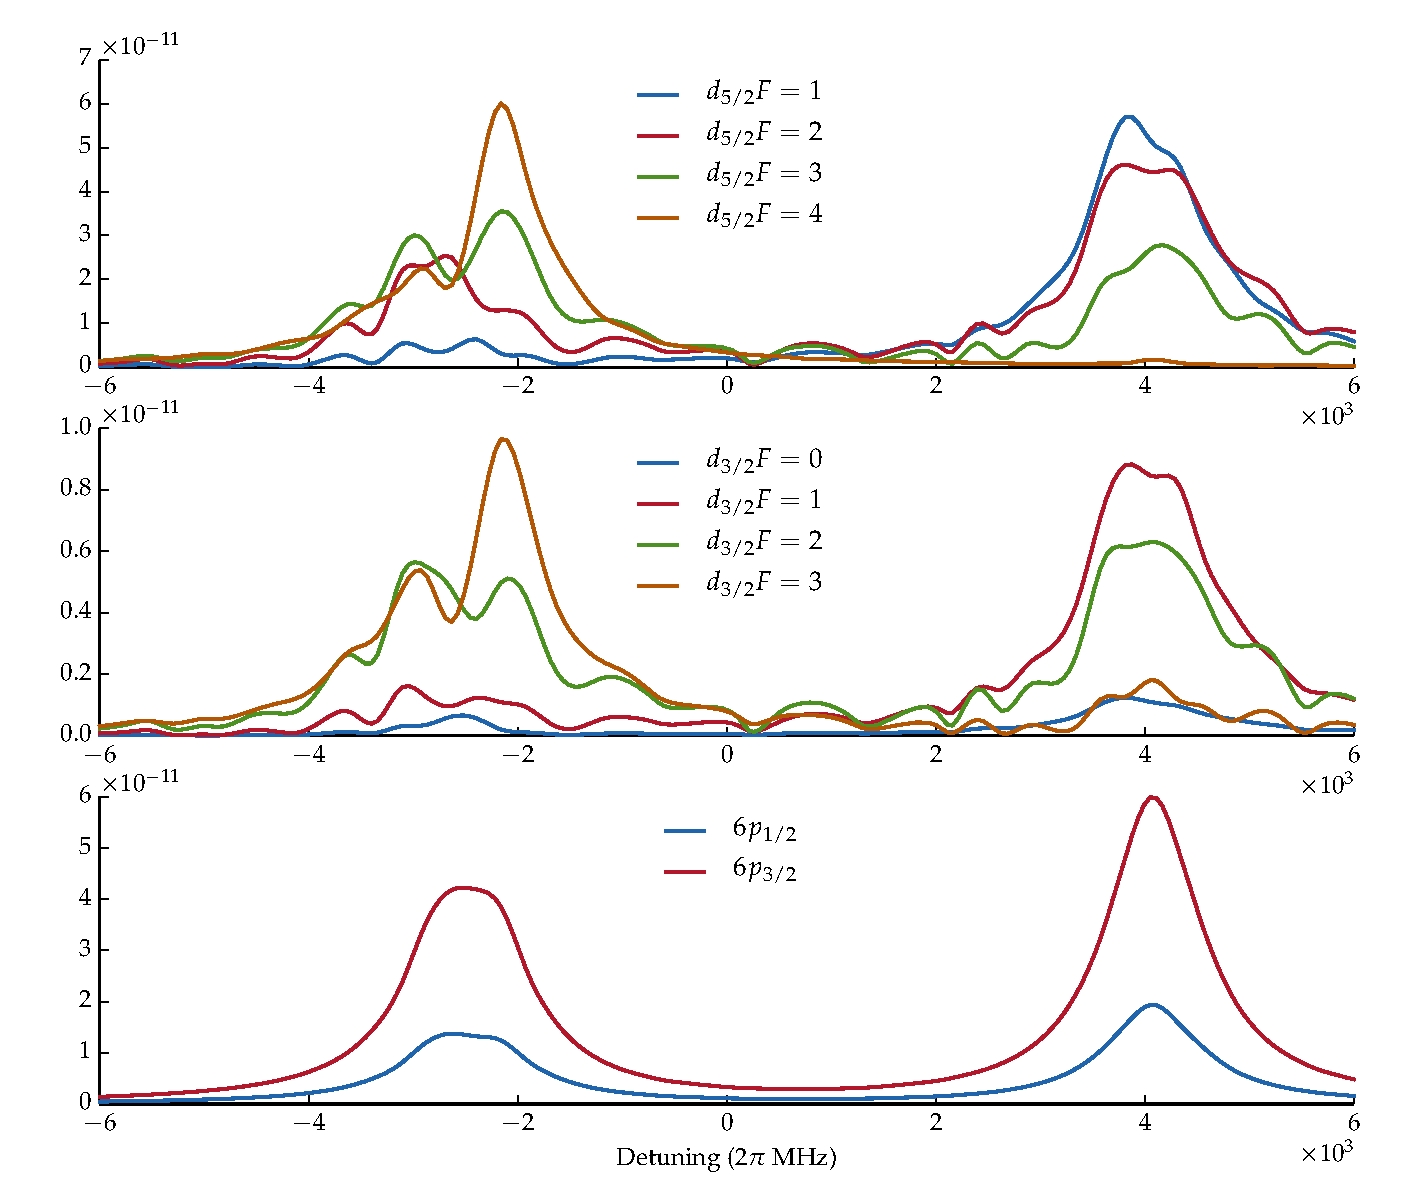
\includegraphics[width=\linewidth]{figs/05_twophoton/rb87_5spd6p_hf_2_solve_scan_e02_FIXED_1e2W_fig2.pdf}
    \caption{
    Populations of the $^{87}$Rb $5\rm{D}_{\nicefrac{5}{2}}$
    (top) and $5\rm{D}_{\nicefrac{3}{2}}$ (middle) excited states, and
    $6\rm{P}$ (bottom) sink states for the same system as in figure 
    \ref{fig:strong_SP_state_pop}.
    }
    \label{fig:strong_D6P_state_pop} 
    \end{figure} 

    In figures \ref{fig:strong_SP_state_pop} and \ref{fig:strong_D6P_state_pop}
    we show the populations of all states for a simulated scan of a stronger
    beam with intensity $I = $ \unit[$10^2$]{W cm$^{-2}$}. At this power the
    individual $5\rm{P}_{\nicefrac{3}{2}}$ excitations overlap and are
    significantly broadened, such that we show all of the \textsc{d2} lines on
    the same plots over a detuning range of \unit[12]{GHz}. We see a small
    amount of population in both of the $5$D manifolds via  two-photon
    excitation, and structure in the $6$P sink states.

    \begin{figure}[h]
    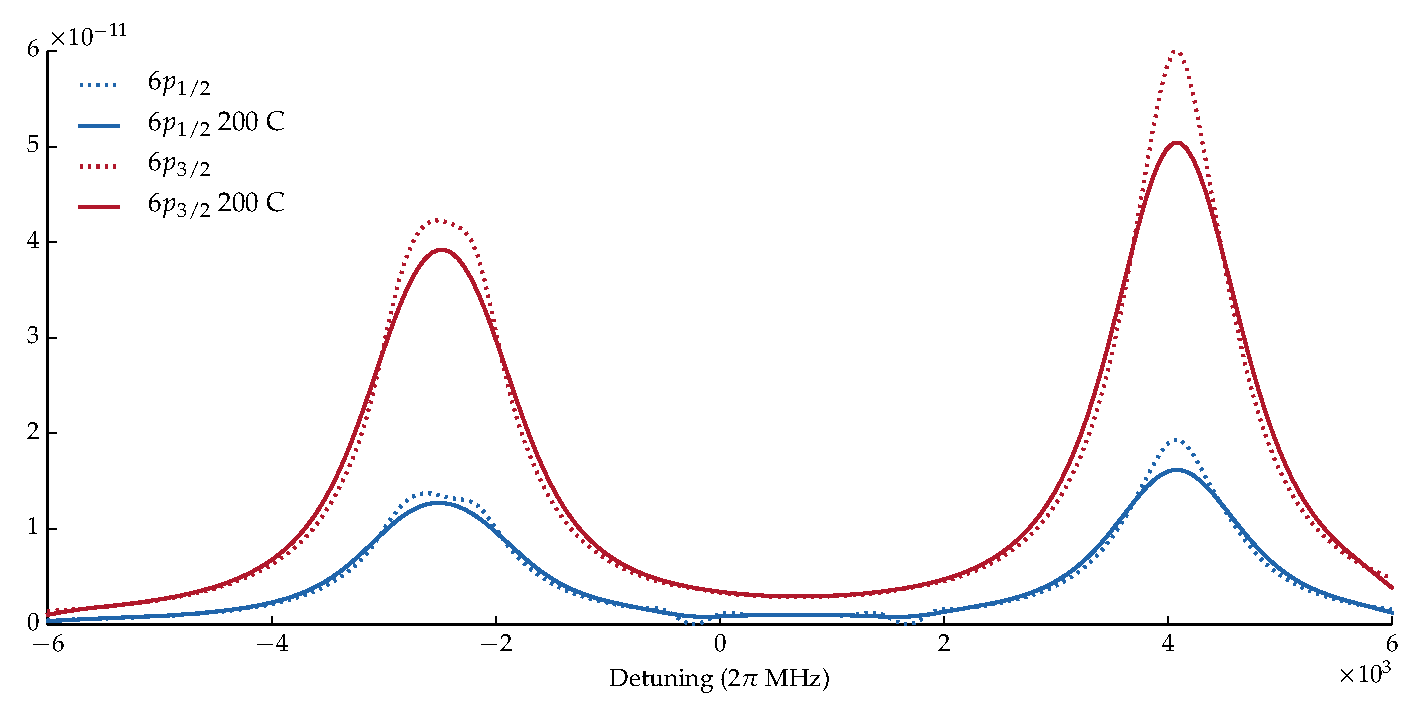
\includegraphics[width=\linewidth]{figs/05_twophoton/rb87_5spd6p_hf_2_solve_scan_e02_FIXED_1e2W_fig9.pdf}
    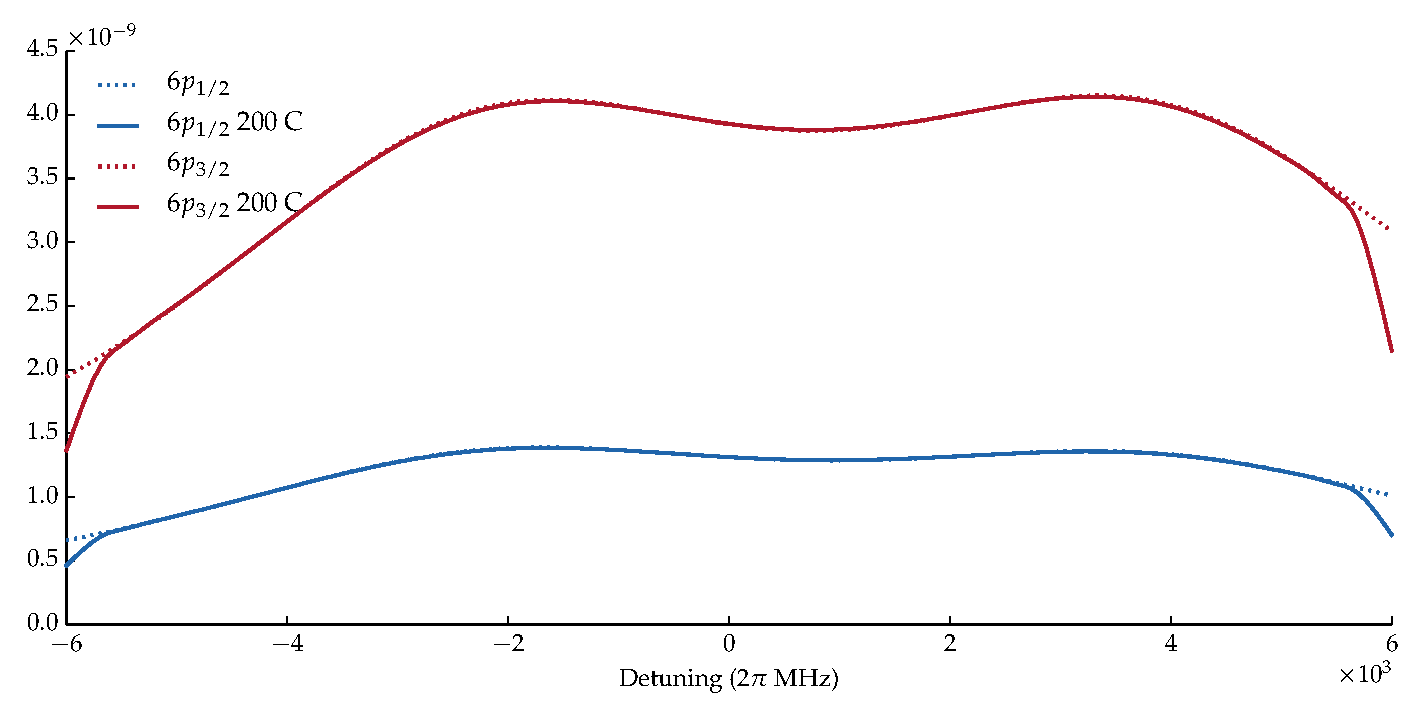
\includegraphics[width=\linewidth]{figs/05_twophoton/rb87_5spd6p_hf_solve_scan_g02_FIXED_fig3.pdf}
    \caption{
    Total populations of the $6\rm{P}_{\nicefrac{1}{2}}$ (blue) and
    $6\rm{P}_{\nicefrac{3}{2}}$ (red) manifolds after \unit[2]{$\mu$s} at $I
    = $ \unit[$10^2$]{W cm$^{-2}$} (top) and $I = $ \unit[$5\times10^3$]{W
    cm$^{-2}$} (bottom). The solid lines represent a \unit[$200$]{\textdegree C}
    Doppler broadened atoms while the dotted represent ultracold (\ie non-
    Doppler broadened) atoms.
    }
    \label{fig:strong_6P_state_pop} 
    \end{figure}    

    In figure \ref{fig:strong_6P_state_pop} we show the effect at two different
    strong beam intensities of including Doppler broadening via a Gaussian
    convolution as described in section \ref{sec:propagation_twolevel}. In this
    case we give and example temperature of \unit[$200$]{\textdegree C}
    corresponding to a number density of $N = \unit[9.26\cdot10^{14}]{m^{-3}}$.
    The doppler width at this temperature is $kv = \unit[2\pi\times385]{MHz}$.
    We see a slight broadening effect at $I = $ \unit[$10^2$]{W cm$^{-2}$} but
    none at $I = $ \unit[$5\times10^3$]{W cm$^{-2}$} as the power broadening
    dominates.

    \begin{figure}[]
    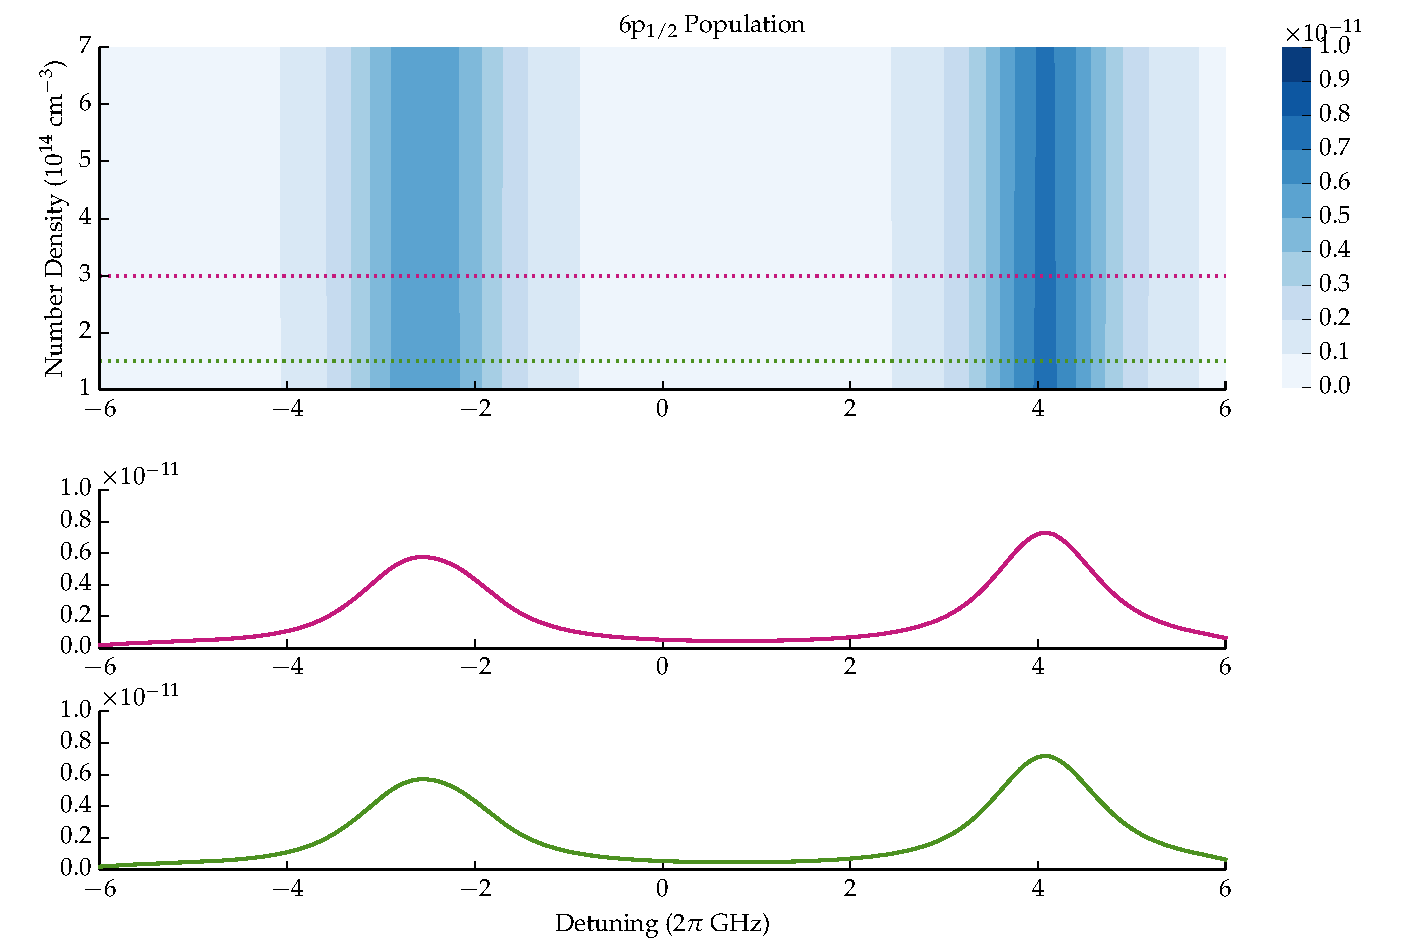
\includegraphics[width=\linewidth]
        {figs/05_twophoton/rb87_5spd6p_hf_solve_scan_f01_fig2.pdf}
    \caption{
    Simulated total population of the $^{87}$Rb
    $6\rm{P}_{\nicefrac{1}{2}}$ sublevels for light input across a GHz detuning
    range covering the \textsc{d2} lines, and over a range of number densities
    $N$ (and thus temperatures $T$).
    }
    \label{fig:blue_plot_model} 
    \end{figure}

    In figure \ref{fig:blue_plot_model} we show the population of the
    $6\rm{P}_{\nicefrac{1}{2}}$ state for $I = \unit[100]{W/cm^2}$, is scanned
    across the full range of the \textsc{d2} lines. At this intensity we see
    that the power broadening is such that the hyperfine structure of the
    excited states is not visible and we see just two peaks representing
    transition from the $F = 1$ and $F = 2$ ground states. The intensity $I =
    \unit[100]{W/cm^2}$ is chosen here becauase the features are on the same
    scale as those seen in the experimental data of figure
    \ref{fig:blue_flourescence}. Power broadening here dominates over Doppler
    broadening.

    The peak population is only on the order of $10^{-11}$, such that we expect
    one in a hundred billion atoms to be excited to the
    $6\rm{P}_{\nicefrac{1}{2}}$, and of the same order in
    $6\rm{P}_{\nicefrac{3}{2}}$, over a duration of \unit[2]{$\mu$s} in the
    beam.
